\documentclass{tufte-handout}

\title{Discrete Probabilistic Programming Languages VI: Sampling\thanks{CS7470 Fall 2023: Foundations of Probabilistic Programming.}}


\newcommand{\varset}[0]{\mathcal{V}}

\author[]{Steven Holtzen\\s.holtzen@northeastern.edu}

%\date{28 March 2010} % without \date command, current date is supplied

%\geometry{showframe} % display margins for debugging page layout
\setcounter{secnumdepth}{1}

\usepackage{graphicx} % allow embedded images
  \setkeys{Gin}{width=\linewidth,totalheight=\textheight,keepaspectratio}
  \graphicspath{{graphics/}} % set of paths to search for images
\usepackage{amsmath,amssymb,amsthm}  % extended mathematics
\usepackage{booktabs} % book-quality tables
\usepackage{units}    % non-stacked fractions and better unit spacing
\usepackage{multicol} % multiple column layout facilities
\usepackage{lipsum}   % filler text
\usepackage{fancyvrb} % extended verbatim environments
  \fvset{fontsize=\normalsize}% default font size for fancy-verbatim environments
\usepackage{listings}
\usepackage{tikz}
\usepackage{mathpartir}
\usepackage{subcaption}
\usepackage{mdframed}
\usepackage{epigraph}
\usepackage{enumitem}
\usepackage{stmaryrd}

\usetikzlibrary{shapes.geometric}


\usepackage[ruled,linesnumbered]{algorithm2e}
\SetKwComment{Comment}{/* }{ */}
\newcommand{\indep}{\perp \!\!\! \perp}

\tikzset{
  treenode/.style = {shape=rectangle, rounded corners,
                     draw, align=center,
                     },
  root/.style     = {treenode, font=\Large, bottom color=red!30},
  env/.style      = {treenode, font=\ttfamily\normalsize},
  dummy/.style    = {circle,draw}
}

% tikz
\usetikzlibrary{patterns,calc,backgrounds}


% TIKZ
\tikzstyle{nnf}=[
  >=stealth,font=\small,auto,scale=0.7,every node/.style={scale=0.7}
]
\tikzstyle{extnode}=[
  draw,circle,inner sep=2pt,fill=white
]

\tikzstyle{leafnode}=[
  draw,fill=gray!20,inner sep=3.5pt
]
\tikzstyle{constnode}=[
  draw,fill=white,inner sep=3.5pt
]
\tikzstyle{label}=[
  fill=white,inner sep=2.5pt
]

\tikzstyle{acarrow}=[
    decoration={markings,mark=at position 1 with {\arrow[scale=0.6]{>}}},
    postaction={decorate},
    shorten >=0.4pt,
    >=latex,
    line width=0.1
]

\tikzstyle{bnarrow}=[
    decoration={markings,mark=at position 1 with {\arrow[scale=1.5]{>}}},
    postaction={decorate},
    shorten >=0.7pt,
    >=latex,
    line width=0.3
]
\tikzstyle{bayesnet}=[
  >=latex, thick, auto
]
\tikzstyle{bnnode}=[
  draw,ellipse,minimum size=7mm,inner sep=1pt,font=\small
]
\tikzstyle{cpt}=[
  font=\footnotesize
]

\tikzstyle{graph}=[
  >=stealth,font=\small,auto,scale=1,every node/.style={scale=1}
]
\tikzstyle{node}=[
  draw,circle,inner sep=3pt,fill=white
]

% BDDs

\tikzstyle{bdd}=[
  >=latex, thick, >=stealth, font=\small,auto,scale=0.9,every node/.style={scale=0.9}
]
\tikzstyle{bddnode}=[
  draw,circle,inner sep=0pt,fill=white,minimum size=5.5mm
]

\tikzstyle{bddtriangle}=[
  draw, regular polygon, regular polygon sides = 3,inner sep=1pt,fill=white,minimum size=5.5mm
]

\tikzstyle{highedge}=[
    line width=0.9
]
\tikzstyle{lowedge}=[
    line width=0.9,dotted
]
\tikzstyle{bddterminal}=[
  draw,fill=gray!20,inner sep=2.5pt, font=\small
]

\lstdefinestyle{compact}{
  \ttfamily\tiny
}


\usetikzlibrary{positioning}

\newtheorem{theorem}{Theorem}
\newtheorem{definition}{Definition}
\newtheorem{conjecture}{Conjecture}
\newtheorem{lemma}{Lemma}
\newtheorem{exercise}{Exercise}
\newtheorem{remark}{Remark}


\usepackage{xcolor}

\definecolor{codegreen}{rgb}{0,0.6,0}
\definecolor{codegray}{rgb}{0.5,0.5,0.5}
\definecolor{codepurple}{rgb}{0.58,0,0.82}
\definecolor{backcolour}{rgb}{0.95,0.95,0.92}

\lstdefinestyle{mystyle}{
    backgroundcolor=\color{backcolour},   
    commentstyle=\color{codegreen},
    keywordstyle=\color{magenta},
    numberstyle=\tiny\color{codegray},
    stringstyle=\color{codepurple},
    basicstyle=\ttfamily\footnotesize,
    breakatwhitespace=false,         
    breaklines=true,                 
    captionpos=b,                    
    keepspaces=true,                 
    numbers=left,                    
    numbersep=5pt,                  
    showspaces=false,                
    showstringspaces=false,
    showtabs=false,                  
    tabsize=2
}

\lstset{style=mystyle}

\newcommand{\defn}[1]{\textbf{#1}}
\newcommand{\dbracket}[1]{\left \llbracket {#1} \right \rrbracket}
\newcommand{\dist}[1]{\mathtt{Dist}(#1)}
\newcommand{\true}[0]{\texttt{true}}
\newcommand{\te}[0]{\texttt{e}}
\newcommand{\false}[0]{\texttt{false}}
\newcommand{\real}[0]{\mathbb{R}}
\newcommand{\rational}[0]{\mathbb{Q}}
\newcommand{\lebesgue}[0]{\mathbb{L}}
\newcommand{\eval}[0]{\mathrm{ev}}
\newcommand{\disc}[0]{\textsc{Disc}}
\newcommand{\borel}[0]{\mathcal{B}}
\newcommand{\ent}[0]{\mathbb{S}}
\newcommand{\prog}[0]{\texttt{p}}
\newcommand{\bool}[0]{\mathbb{B}}
\newcommand{\cont}[0]{\textsc{Cont}}
\newcommand{\prop}[0]{\textsc{Prop}}
\newcommand{\bdd}[0]{\textsc{Bdd}}
\newcommand{\robdd}[0]{\textsc{Robdd}}
\newcommand{\compiles}[0]{\rightsquigarrow}

\newcommand{\bddtriangle}[1]{
    \begin{tikzpicture}
    \node [bddtriangle] {#1};
    \end{tikzpicture}}
\newcommand{\bddtrue}[0]{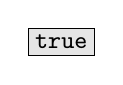
\begin{tikzpicture}
      \node [bddterminal] {$\true$};
    \end{tikzpicture}}
\newcommand{\bddfalse}[0]{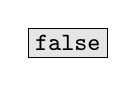
\begin{tikzpicture}
      \node [bddterminal] {$\false$};
    \end{tikzpicture}}


% Standardize command font styles and environments
\newcommand{\doccmd}[1]{\texttt{\textbackslash#1}}% command name -- adds backslash automatically
\newcommand{\docopt}[1]{\ensuremath{\langle}\textrm{\textit{#1}}\ensuremath{\rangle}}% optional command argument
\newcommand{\docarg}[1]{\textrm{\textit{#1}}}% (required) command argument
\newcommand{\docenv}[1]{\textsf{#1}}% environment name
\newcommand{\docpkg}[1]{\texttt{#1}}% package name
\newcommand{\doccls}[1]{\texttt{#1}}% document class name
\newcommand{\docclsopt}[1]{\texttt{#1}}% document class option name
\newenvironment{docspec}{\begin{quote}\noindent}{\end{quote}}% command specification environment



\begin{document}
\maketitle% this prints the handout title, author, and date

Some logistics:
\begin{itemize}
  \item Next week is Systems Week. Have a look at the systems week page! Start playing with 
  some existing PPL systems.
  \item I am happy to meet about your project. Proposal is due Oct. 20.
\end{itemize}

\section{Sampling \& approximate reasoning}
\begin{itemize}
  \item Up until now we have been exclusively discussing \emph{exact reasoning}:
  computing the exact probability that a program will output a particular value

  \item Problems with exact reasoning:
  \begin{itemize}
    \item State-space explosion
    \item Limited expressive power: how can we handle continuous probability, or loops that may never terminate?
    \item ``All-or-nothing'': exact answer or nothing at all
  \end{itemize}

  \item An alternative is \emph{approximate reasoning}. Many of the most popular PPLs in use 
  today support exclusively this mode of reasoning.\sidenote{For example, Stan~\citep{carpenter2017stan}.}

  \item There is an entirely separate school of PPLs that reason by \emph{sampling}.

  \item The crucial mechanism is the \emph{sample mean}, which gives an estimate of the expectation 
  of a random variable:
  
  \begin{definition}[Expectation]
    Let $(\Omega, \Pr)$ be a probability space and $f : \Omega \rightarrow
    \real$ be a random variable. The \emph{expectation} (or \emph{average value}) of $f$ with respect to 
    $\Pr$ is defined:
    \begin{align}
      \E_{\Pr[f]} \triangleq \sum_{\omega \in \Omega} \Pr(\omega) f(\omega).
    \end{align}
  \end{definition}

  \begin{definition}[Sample mean]
    Let $(\Omega, \Pr)$ be a probability space and $f : \Omega \rightarrow
    \real$ be a random variable. Then, the \emph{sample mean} of $f$ 
    with $N$ samples is defined:
    \begin{align}
      \frac{1}{N} \sum_{\omega_i \sim \Pr}^N f(\omega_i),
    \end{align}
    where the notation $\omega_i \sim \Pr$ denotes drawing a sample $\omega_i$ from 
    the probability distribution $\Pr$.
  \end{definition}

  \marginnote{One may wonder \emph{how quickly} a particular
  estimate of the mean approaches the true value (i.e., how many samples one
  must draw in order to have an accurate estimate with high probability). There
  are many bounds of this sort known broadly as \emph{concentration
  inequalities}; \citet{shalev2014understanding} has a nice summary of some 
  of the useful concentration inequalities that arise in practice in the appendix.}

  \item The reason why we use the sample estimator is that the \emph{law of large numbers} 
  guarantees that, as $N \rightarrow \infty$, the sample mean approaches the 
  expectation, i.e.:
  \begin{align}
    \lim_{N \rightarrow \infty} \frac{1}{N} \sum_{\omega_i \sim \Pr}^N f(\omega_i) = \E_{\Pr}[f].
  \end{align}

  \item What will do is give a semantics to programs in terms of expectations, and then 
  use the expectation estimator in order to get an approximation for the program's 
  behavior

\end{itemize}

\section{Sampling semantics for \disc{}}
\marginnote{This secton is based on the semantics given by \citet{culpepper2017contextual}.}
\begin{itemize}
  \item \textbf{Goal}: Give a semantics that draws samples from
  $\dbracket{\te}$, where $\te$ is a (probabilistic) \disc{} term. Then, we can
  use the sample mean to approximate the semantics of a probabilistic program.

  \item We still want our semantics to be a \emph{deterministic relation} on terms; how can 
  we draw samples using a deterministic relation?

  \item Solution: Add a \emph{source of randomness} to our context (just like how your 
  computer has \texttt{/dev/rand})

  \item To get our feet wet with this new style of semantics, let's consider a
  tiny sub-language of \disc{} with only the following syntax with only fair
  coin-flips and no observations:
\begin{lstlisting}[mathescape=true]
  e ::= flip 1/2 | x $\leftarrow$ e; e | x | e $\land$ e | e $\lor$ e | $\neg$ e
\end{lstlisting}

  The denotation of this sub-language is inherited from \disc{}. 

  \item To draw samples from this language, we add to our evaluation judgment an
  \emph{finite stream of fair coin-flips} $\sigma \in \bool^{k}$ for some integer 
  $k$. 
  
  \item To handle binding, we will need a way to split this bit-stream up. We
  notate this $\pi_L$ and $\pi_R$, which split $\sigma$ into two disjoint random
  sets of bits. We can define these projections in a number of ways, but a
  simple way is to define $\pi_R$ to take all even bits and $\pi_L$ to take all
  odd bits:
  \begin{align*}
    \pi_R(v_1, v_2, v_3, \dots) \triangleq (v_2, v_4, v_6, ...) \quad 
    \pi_L(v_1, v_2, v_3, \dots) \triangleq (v_1, v_3, v_5, ...)
  \end{align*}

  \item Then we can define a judgment $\sigma \vdash \te \Downarrow^S v$:

  \begin{mathpar}
    \inferrule{}{v :: \sigma \vdash \texttt{flip} \Downarrow^S v}
    \and
    \inferrule{\pi_L(\sigma) \vdash \te_1 \Downarrow^S v_1 \and 
    \pi_R(\sigma) \vdash \te_2[v_1/x] \Downarrow^S v_2
    }{\sigma \vdash x \leftarrow \te_1; \te_2 \Downarrow^S v_2}
  \end{mathpar}

  This judgment simply gets \emph{stuck} if there are not enough coin flips in
  our context.

  \item Since our semantics are deterministic, can define a function $ev(\sigma,
  \te)$ that produces the value that the (closed) term $\te$ evaluates to for
  $\sigma$:


  \item Now we can establish an adequacy condition that relates an expectation 
  (over finite sequences of coin tosses) to the denotation:
  
  \begin{theorem}
  Let $\Pr$ be the distribution on the finite bit streams $\bool^k$, and furthermore assume 
  that $k$ is ``big enough''.\sidenote{What does it mean for $k$ to be big enough? Formally, 
  we assume that $k > 2^n$, where $n$ is the number of bindings in the term.} Assume
  $\Gamma \vdash \te$.  Then, for any $\gamma \in \dbracket{\Gamma}$,
  $\E_{\sigma \sim \Pr}[\mathbb{1}(ev(\sigma, \te[\gamma]) = \true)] =
  \dbracket{\te[\gamma]}(\true)$.
  \end{theorem}
  \begin{proof}
  The non-probabilistic cases are straightforward. Let's see the \texttt{flip} 
  case first. We can disregard $\gamma$ since this term is closed.
  \begin{fullwidth}
  \begin{align*}
    \E_{\sigma \sim \Pr}[\mathbb{1}(ev(\sigma, \texttt{flip}~1/2))] &= 
    \sum_{(v_1, v_2, \dots, v_k)} \Pr(v_1, v_2, \cdots, v_k) \mathbb{1}[ev((v_1, \dots, v_k), \texttt{flip}~1/2) = \true)] \\ 
    &= \sum_{v_2, \dots, v_k} \Pr(v_2, \dots, v_k) \times \sum_{v_1} \Pr(v_1) \mathbb{1}[ev(v_1, \texttt{flip}~1/2) = \true)] \\ 
    % &= \Pr(\sigma) \sum_{v} \Pr(v::\sigma) \mathbb{1}[ev(v::\sigma, \te) = \true)]   \\
    &= \Pr(v = \true) \mathbb{1}[\true = \true] + \Pr(v = \false)\mathbb{1}[\false = \true] \\ 
    &= 1/2  \\
    &= \dbracket{\texttt{flip~1/2}}(\true).
  \end{align*}
  \end{fullwidth}

  Now for the bind case, $x \leftarrow \te_1; \te_2$. Assume by induction that:
  \begin{itemize}
    \item $\E_{\sigma \sim \Pr}[\mathbb{1}(ev(\sigma, \te_1) = \true)] = \dbracket{\te_1}(\true)$.
    \item $\E_{\sigma \sim \Pr}[\mathbb{1}(ev(\sigma, \te_2) = \true)] = \dbracket{\te_2}(\true)$.
  \end{itemize}
  Proceeding:
  \begin{fullwidth}
  \begin{align}
    \E_{\sigma \sim \Pr}[\mathbb{1}(ev(x \leftarrow \te_1; \te_2) = \true)] 
    &= \sum_{\sigma} \Pr(\sigma) \mathbb{1}(ev(x \leftarrow \te_1; \te_2) = \true) \\ 
    &= \sum_\sigma \Pr(\sigma) \sum_v \mathbb{1}[ev(\te_1, \pi_R(\sigma)) = v] \mathbf{1}[ev(\te_2[v/x], \pi_R(\sigma)) = \true] \\ 
    &= \sum_{v_1, v_3, \dots}  \Pr(v_1, v_3, \dots) [ev(\te_1, v_1, v_3, \dots) = v]  \times \sum_{v_2, v_4, \dots} \Pr(\sigma) \mathbb{1}[ev(\te_2[v/x], \sigma) = \true]~\mathrm{d}\sigma\\
    &= \sum_v \dbracket{\te_1}(v) \dbracket{\te_2[v/x]}(\true).
  \end{align}
\end{fullwidth}
   
  This final equality holds due to a natural Kripke-esque monotonicity property.
  \end{proof}

  \item This directly gives us a procedure for sampling
\end{itemize}

\subsection{Infinite streams}

\begin{itemize}
  \item \textbf{Problem}: How do we know how many coins to draw a-priori?

  \item One solution is to draw samples from an
  \emph{infinite stream of fair coin-flips} $\sigma \in \bool^{\nat}$.

  \item Given access to this context, we can define a relation $\sigma \vdash
  \te \Downarrow^S v$ for our tiny language above (showing only the probabilistic terms):
  \begin{mathpar}
    \inferrule{}{v :: \sigma \vdash \texttt{flip} \Downarrow^S v}
    \and
    \inferrule{\pi_L(\sigma) \vdash \te_1 \Downarrow^S v_1 \and 
    \pi_R(\sigma) \vdash \te_2[v_1/x] \Downarrow^S v_2
    }{\sigma \vdash x \leftarrow \te_1; \te_2 \Downarrow^S v_2}
  \end{mathpar}

  \item Now we can run our program for different values of $\sigma$:
  \footnotesize{
  \begin{mathpar}
    \inferrule{\true :: \pi_L(\sigma) \vdash \texttt{flip}~1/2 \Downarrow^S \true 
    \and 
    \inferrule{\false :: \pi_L(\pi_R(\sigma)) \vdash \texttt{flip}~1/2 \Downarrow^S \false \and 
      \inferrule{\inferrule{\dots}{\pi_R(\pi_R(\sigma)) \vdash \true \lor \false \Downarrow^S \true}}{\pi_R(\pi_R(\sigma)) \vdash \texttt{return}~\true \lor \false \Downarrow^S \true}
    }
    {y \leftarrow \texttt{flip}~1/2; \texttt{return }\true \lor y \Downarrow^S \true}
    }
    {\true :: \false :: \sigma \vdash x \leftarrow \texttt{flip}~1/2; y \leftarrow \texttt{flip}~1/2; \texttt{return }x \lor y \Downarrow^S \true}
  \end{mathpar}
  }
\end{itemize}

\section{Adequacy}
\begin{itemize}
  \item \textbf{Goal}: Prove the sampling relation $\sigma \vdash \te
  \Downarrow^S v$ ``correctly sample'' from $\dbracket{\te}$.

  \item To make this formal, we will need a way of representing a probability
  distribution on $\bool^\nat$.  This is actually much trickier to define than
  it seems at first! 

  Let's start by defining the probability of any \emph{finite subsequence} of bits; we 
  will refine this notion more later:
  \begin{align}
    \Pr((v_1, v_2, \dots, v_n)) = \frac{1}{2^n}
  \end{align}
  
  % We will assume that standard properties of probability distributions (such as marginalization)
  % hold of $\Pr$, for instance:
  % \begin{align}
  %   \sum_{(v_2, v_3, v_4, \dots) \in \bool^\nat}\Pr(v_1 = \true, v_2, v_3, v_4, \dots) = 1/2
  % \end{align}


\end{itemize}


\begin{theorem}
  Let $\Pr$ be the distribution on the infinite bit streams $\bool^\nat$. Assume $\Gamma \vdash \te$.
  Then, for any $\gamma \in \dbracket{\Gamma}$,
  $\E_{\sigma \sim \Pr}[\mathbb{1}(ev(\sigma, \te[\gamma]) = \true)] = \dbracket{\te[\gamma]}(\true)$.
\end{theorem}
\begin{proof}
  The non-probabilistic cases are straightforward. Let's see the \texttt{flip} 
  case first. We can disregard $\gamma$ since this term is closed.
  \begin{align*}
    \E_{\sigma \sim \Pr}[\mathbb{1}(ev(\sigma, \te))] &= 
    \int \Pr(v::\sigma) \mathbb{1}[ev(v::\sigma, \te) = \true)]~\mathrm{d}\sigma \\ 
    &= \Pr(v = \true) \mathbb{1}[\true = \true] + \Pr(v = \false)\mathbb{1}[\false = \true] \\ 
    &= 1/2 = \dbracket{\texttt{flip~1/2}}(\true).
  \end{align*}

  Now for the bind case, $x \leftarrow \te_1; \te_2$. Assume by induction that:
  \begin{itemize}
    \item $\E_{\sigma \sim \Pr}[\mathbb{1}(ev(\sigma, \te_1) = \true)] = \dbracket{\te_1}(\true)$.
    \item $\E_{\sigma \sim \Pr}[\mathbb{1}(ev(\sigma, \te_2) = \true)] = \dbracket{\te_2}(\true)$.
  \end{itemize}
  Proceeding:
  \begin{fullwidth}
  \begin{align}
    \E_{\sigma \sim \Pr}[\mathbb{1}(ev(x \leftarrow \te_1; \te_2) = \true)] 
    &= \int \Pr(\sigma) \mathbb{1}(ev(x \leftarrow \te_1; \te_2) = \true)~\mathrm{d}\sigma \\ 
    &= \int \Pr(\sigma) \sum_v \mathbb{1}[ev(\te_1, \pi_R(\sigma)) = v] \mathbf{1}[ev(\te_2[v/x], \pi_R(\sigma)) = \true]~\mathrm{d}\sigma \\ 
    &= \sum_v \int \Pr(\sigma) [ev(\te_1, \sigma) = v]~\mathrm{d}\sigma \times \int \Pr(\sigma) \mathbb{1}[ev(\te_2[v/x], \sigma) = \true]~\mathrm{d}\sigma\\
    &= \sum_v \dbracket{\te_1}(v) \dbracket{\te_2[v/x]}(\true).
  \end{align}
\end{fullwidth}
\end{proof}

\begin{itemize}
  \item Now we are left with one final problem: how can we ``run these
  semantics'' on a computer?  I.e., how can we effectively sample from an
  infinite stream of random bits, which seems to require infinite memory (and in
  which each sample has probability 0)? We can \emph{sample the bits lazily}: 
  each time a fresh random bit is required, flip a fair coin to sample it.

  \item Now, let's compare sampling against exact: when might one prefer 
  sampling over exact, and vise versa?
\end{itemize}



\subsection{The uniform distribution on infinite bit streams}
\begin{itemize}
  \item \textbf{Goal}: Define the probability space $(\bool^\nat, \Pr)$
  \item \textbf{Problem}: It is surprisingly hard to give a formal 
  description of this space! Observe: every $\sigma \in \bool^\nat$ 
  has a probability of 0. This seems broken.
  \item We will need to venture into the machinery of \emph{measure theory}
  to give a formal description of this probability distribution.\marginnote{Some recommended
  measure theory textbooks: \citet{axler2020measure,rosenthal2006first,pollard2002user}.}
  \item We need a new definition of probability space. The main insight 
  is that, while individual elements of the sample space might have 0 probability,
  \emph{events} may not have 0 probability. For instance, consider the event $A_1$ 
  which is the collection of all infinite bit-streams that begin with the first 
  bit being $\true$:
  \begin{align*}
    A_1 = \{\true, a_1, a_2, \dots \}
  \end{align*}
  Intuitively, this event should have probability 1/2, $\Pr(A_1) = 1/2$, even though 
  every individual element of the sample space inside it has probability 0.

  \item How do we resolve this paradox? We introduce a new \emph{structure on events}, 
  and define our probability \emph{measure} on that event structure instead of 
  directly on the sample space.

  \begin{definition}
    Let $\Omega$ be a sample space.
    A \emph{$\sigma$-algebra} $\calF$ on $\Omega$ is a collection of subsets of
    $\Omega$ that:
    \begin{enumerate}
      \item Contains $\Omega$;
      \item Is closed under complementation: if $A \in \calF$ then $\overline{A} \in \calF$;
      \item Is closed under countable union: If $\{A_i\} \in \calF$, then $\bigcup_i A_i \in \calF$.
    \end{enumerate}
  \end{definition}

  \item The simplest kind of $\sigma$ algebra is the \emph{power-set
  $\sigma$-algebra}. Let $\Omega$ be a finite set, and $2^\Omega$ be the set of
  all subsets formed out of $\Omega$. Then, $2^\Omega$ is a $\sigma$-algebra.

  \item Now we can define a generalized probability space:
  \begin{definition}
    Let $\Omega$ be a sample space, $\calF$ be a $\sigma$-algebra on $\Omega$, and 
    $\mu : \calF \rightarrow [0,1]$ be a map. We call $\mu$ a \emph{probability measure} 
    if it satisfies:
    \begin{enumerate}
      \item $\mu(\Omega) = 1$;
      \item Countable additivity: for disjoint $\{A_i\} \in \calF$, it holds that 
      $\mu(\bigcup_i A_i) = \sum_i \mu(A_i)$.
    \end{enumerate}
    We call the triple $(\Omega, \calF, \mu)$ a \emph{probability space}.
  \end{definition}

  \item Note: up until now, we have been implicitly working in a finite probability 
  space where $\Omega$ is finite, $\calF$ is the power-set $\sigma$-algebra, and 
  $\mu$ is defined only on $\omega \in \Omega$. We can extend this old definition to a 
  generalized probability space by countable additivity.

  \marginnote{See \citet[Section 2.6]{rosenthal2006first} for a detailed discussion on 
  coin-flipping measures.}

  \item Now the key step for resolving our coin-flipping dilemma: we define a
  collection of events and their probability measure according to our intuition
  about how finite sequences of coin tosses behave:
  \begin{align}
    \mathcal{J} = \{A_{a_1a_2 \dots a_n} \mid n \in \nat, a_i \in \{0, 1\} \} \cup \{\emptyset, \Omega\}
  \end{align}
  Then, for any $A_{a_1, a_2, \dots, a_n} \in \mathcal{J}$, we define $\mu(A_{a_1, a_2, \dots, a_n}) = 1/2^n$, 
  $\mu(\emptyset) = 0, \mu(\Omega) = 1$.

  \item Clearly $\mathcal{J}$ is not yet a $\sigma$-algebra (it is not closed
  under countable unions), and $\mu$ is not a fully-defined probability 
  measure since it is not defined on a valid $\sigma$-algebra. \sidenote{The set 
  $\mathcal{J}$ is what is known as a \emph{semi-algebra} on $\Omega$: it is a collection 
  of subsets of $\Omega$ that contains $\emptyset$ and 
  $\Omega$, is closed under \emph{finite} intersection, and the complement of any element 
  is equal to a \emph{finite} disjoint union of elements.}
  So, let's define 
  $\mu$ to satisfy countable additivity. Let $\{A_i\}$ be disjoint elements of $\mathcal{J}$. 
  Then, we define:
  \begin{align}
    \mu\left( \bigcup_{i} A_i \right) = \sum_{i} \mu(A_i).
  \end{align}
  \item Now, there is a well-known theorem in measure theory called the
  \emph{extension theorem} that says that (1) there exists a sigma algebra
  $\cal$ that contains $\mathcal{J}$; and (2) there is a countably additive
  probability measure $\mu^*$ on $\calF$ that agrees with $\mu$ above, i.e. for
  any $A \in \mathcal{J}$, we have that $\mu^*(A) = \mu(A)$.

  \item This resolves all of our paradoxes: we now have a probability measure that 
  lets us (1) reason about probabilities of finite subsequences; (2) assigns 
  zero probability to all infinite sequences
\end{itemize}

\bibliographystyle{plainnat}
\bibliography{../bib}


\end{document}